% =====================================================================
%  chapter02_city_mapping.tex — מיפוי שטח
% =====================================================================
\chapter{מיפוי שטח}
\chaptersubtitle{הגיאוגרפיה של גינות כלבים ופינות הצל הנכונות}

\section{המפה שבראש של הכלב}
לכם יש \en{Waze}. לכלב יש מפה אחרת לגמרי: איפה העץ שכולם מסמנים, איפה הברזייה, איפה החתול
שיושב על הגדר ואיפה המדרכה שבקיץ שורפת את הכפות. בעלי כלבים ותיקים מפתחים עם הזמן מפה כפולה,
שמשלבת את מה שנוח לבני אדם עם מה שבטוח ומעניין לכלב. הפרק הזה עוזר לבנות אותה בכוונה ולא רק
בדרך של ניסוי וטעייה.

\begin{figure}[h]
  \centering
  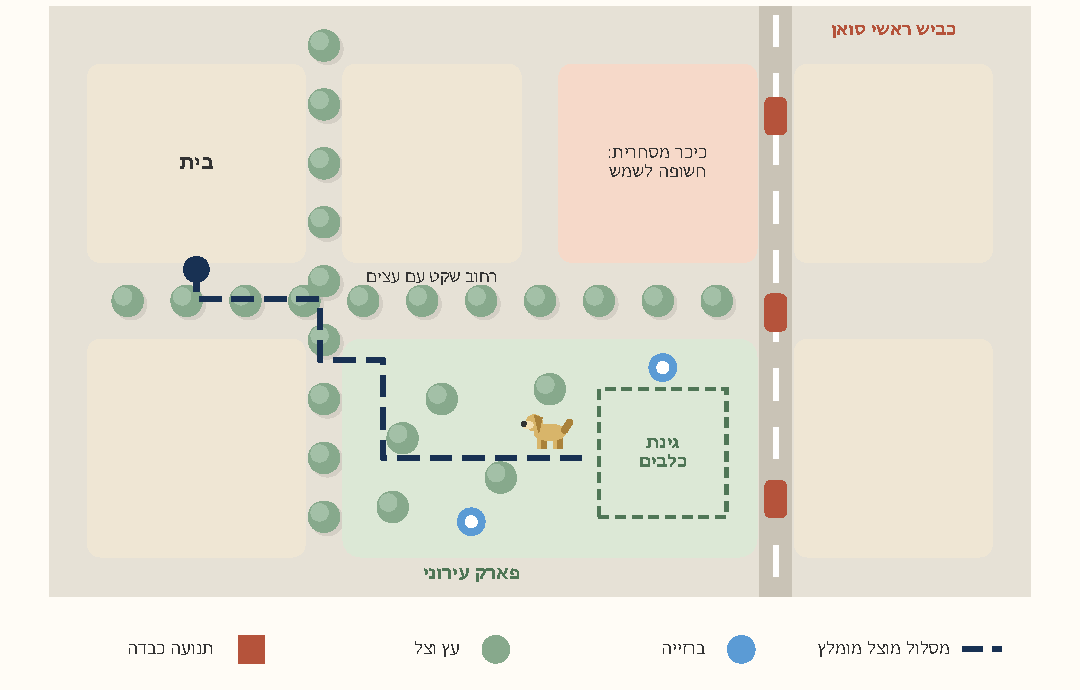
\includegraphics[width=0.86\linewidth]{original_neighborhood_map.pdf}
  \caption{מפת שכונה קונספטואלית: מסלול מוצל מהבית לגינת הכלבים, הרחק מהכביש הסואן ומהכיכר
  החשופה. איור מקורי שנוצר בקוד \en{Python} (\en{matplotlib}) מצורות גאומטריות. השכונה בדיונית.}
  \label{fig:map}
\end{figure}

\section{חמש שאלות לפני שבוחרים מסלול}
\begin{enumerate}[label=\textbf{\arabic*.},leftmargin=*]
  \item \textbf{צל:} כמה מהמסלול עובר מתחת לעצים או בצד המוצל של הרחוב, בשעה שבה אתם יוצאים?
  \item \textbf{מים:} יש ברזייה בדרך? אם לא, אתם המים. על זה בפרק 3.
  \item \textbf{משטח:} אספלט, אבן, דשא או חול? משטחים כהים וחשופים מתחממים מאוד בשמש.
  \item \textbf{תנועה:} כמה מעברי חציה, כמה כבישים ראשיים, וכמה אופניים וקורקינטים במדרכה?
  \item \textbf{עומס:} כמה אנשים, כלבים ורעש יש במסלול בשעה הזאת? לכלב רגיש, שקט שווה יותר מקיצור דרך.
\end{enumerate}

\section{מדרכה חמה, כפות רגישות}
בימים חמים האספלט יכול להתחמם הרבה יותר מהאוויר, ואיגוד הווטרינרים האמריקאי (\en{AVMA}) מזהיר
שמשטחים חמים עלולים לגרום לכוויות בכפות. הוא ממליץ להגביל פעילות בימים חמים, לדאוג לצל ולמים
ולהעדיף את השעות הקרירות של היום \cite{avma-warm}. מחקר על כלבים בבריטניה מצא שפעילות גופנית
היא אחד הגורמים השכיחים למכת חום בכלבים, ושהסיכון גבוה יותר בכלבים ברכיצפליים (בעלי אף קצר), בכלבים
כבדים ובכלבים מבוגרים \cite{hall2020}.

\begin{notebox}
בדיקה מעשית שנפוצה בקרב בעלי כלבים: הניחו את גב כף היד על המדרכה לכמה שניות. אם לא נוח לכם
להשאיר אותה שם, כנראה שזה חם מדי גם לכפות. זו בדיקה גסה, לא מדידה. בימים חמים במיוחד
עדיף לקצר, ללכת על דשא או בצל, או לדחות את הטיול לשעה קרירה יותר.
\end{notebox}

\section{גינת כלבים או רחוב שקט?}
גינת כלבים היא מקום נהדר לכלב חברותי שאוהב לרוץ, אבל היא לא חובה, ולא כל כלב נהנה בה.
כשבודקים גינה, כדאי להסתכל על הגדר והשער הכפול, על הצל ועל המים, על מספר הכלבים בשעה
שבה אתם מגיעים ועל ההתנהגות של הבעלים: האם מישהו בכלל מסתכל על הכלב שלו?

\begin{table}[h]
\centering
\caption{השוואה בין סביבות הליכה עירוניות (הערכה כללית, משתנה משכונה לשכונה)}
\label{tab:areas}
\renewcommand{\arraystretch}{1.35}
\small
\begin{tabularx}{\linewidth}{>{\sffamily\bfseries\color{navy}}p{2.1cm} X X X}
\toprule
{\sffamily\bfseries סוג אזור} & {\sffamily\bfseries יתרונות} & {\sffamily\bfseries אתגרים} & {\sffamily\bfseries מתי כדאי לבחור בו} \\
\midrule
פארק עירוני & שטח פתוח, דשא, עצים ולרוב גם ברזיות & רוכבי אופניים, פיקניקים ושאריות אוכל & טיול ארוך בבוקר או לפני השקיעה \\
\rowcolor{sage!10}
רחוב שקט & מעט רעש ותנועה, קל לשמור על קשב & לעיתים מעט צל, מכוניות חונות שמסתירות שדה ראייה & טיול קצר, כלב רגיש או גור בתחילת הדרך \\
גינת כלבים & ריצה חופשית במרחב מגודר ומפגש חברתי & צפיפות, מתחים בין כלבים, צל ומים לא תמיד זמינים & כלב חברותי, בשעות פחות עמוסות \\
\rowcolor{sage!10}
טיילת & מסלול ארוך ורציף, נוף ורוח & חשיפה לשמש, הרבה אנשים, אופניים וקורקינטים & ערב או בוקר מוקדם, כשהמשטח קריר \\
אזור מסחרי & הרגלה לגירויים, סידורים בדרך & רעש, צפיפות, אוכל על הרצפה ומדרכות חמות & אימון קצר ומבוקר, לא כטיול עיקרי \\
\bottomrule
\end{tabularx}
\end{table}

\section{לחיות ביחד במרחב הציבורי}
העיר שייכת לכולם, גם למי שמפחד מכלבים. בישראל, החוק להסדרת הפיקוח על כלבים קובע כללים להחזקת
כלבים במרחב הציבורי, ובהם חובת רצועה \cite{il-doglaw2002}. בנוסף, לרשויות המקומיות יש חוקי עזר
משלהן, למשל לגבי איסוף צואה ואזורים שבהם מותר לשחרר כלבים. לכן כדאי לבדוק באתר העירייה שלכם מה
חל בשכונה. אוספים כל צואה, מקצרים את הרצועה ליד ילדים, רוכבים ושולחנות של בתי קפה, וזוכרים
שהכלב שלכם הוא השגריר של כל בעלי הכלבים ברחוב.

\begin{fieldbox}
בנו לעצמכם שלושה מסלולים קבועים: \textbf{קצר} לימים עמוסים, \textbf{מוצל} לימים חמים
ו\textbf{ארוך} לסופי שבוע. כשמזג האוויר או מצב הרוח משתנים, לא צריך לתכנן מחדש, רק לבחור.
\end{fieldbox}
